
% drawio link: https://drive.google.com/open?id=10yQD3nL_LmK5xsChKugc4OlRGO5AMMoz
\begin{figure*}[!t]
    \centering
    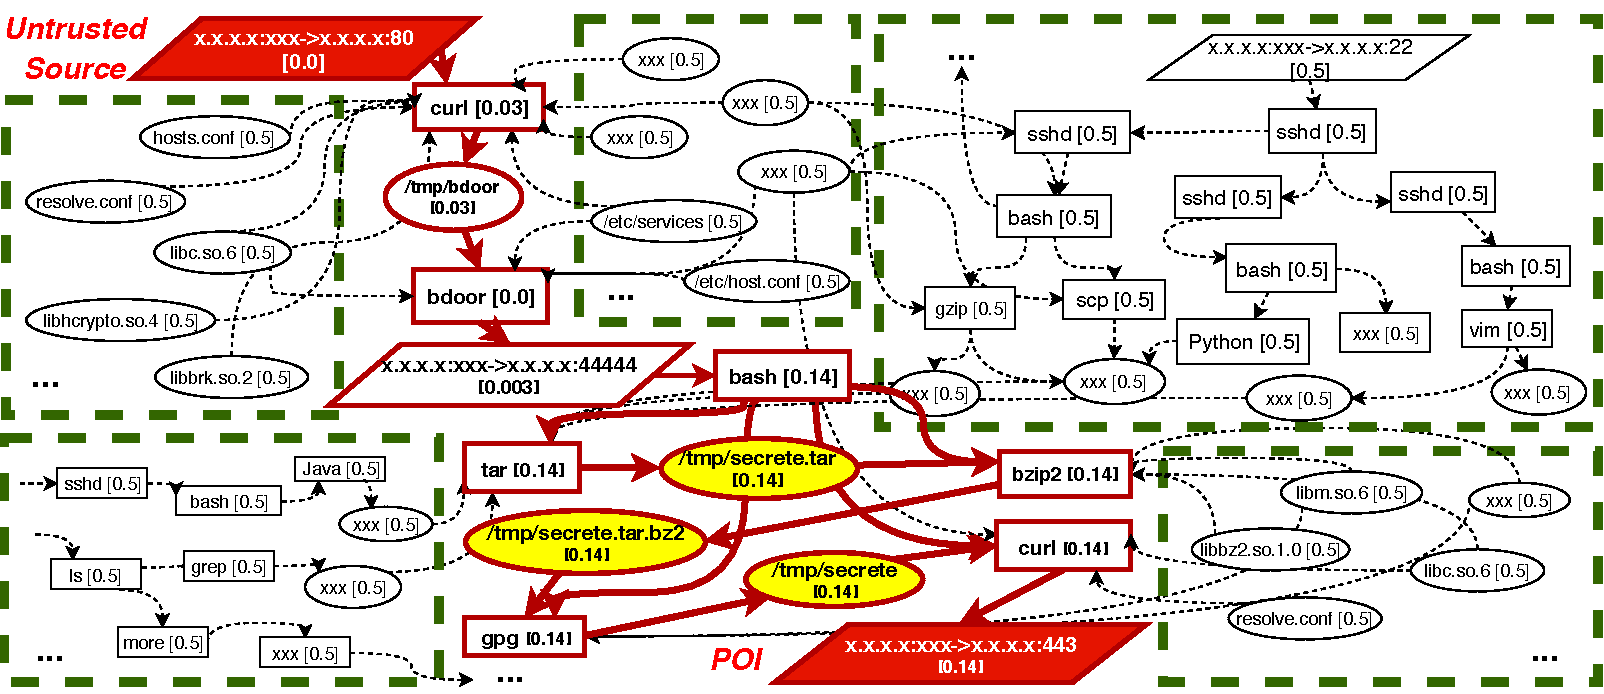
\includegraphics[width=0.94\textwidth]{figs/overview.pdf}
    \caption{Partial dependency graph of a motivating data leakage attack case (rectangles for processes, ovals for files, parallelograms for network connections, yellow ovals for files leaked in this attack).
    The complete dependency graph constructed from the POI (red parallelogram at the bottom) via backward causality analysis contains 106 nodes and 237 edges.
    %
    The untrusted network connection (red parallelogram at the top left) is the root cause node of the POI. %identified by \tool. 
    Critical edges 
    %revealed by \tool 
    that represent the attack sequence are represented by solid red arrows, and nodes on the attack sequence have red frames. 
    Non-critical edges are represented by dashed arrows, and non-critical nodes such as normal activities and system libraries are organized in dashed green rectangles.
    %
    As we can see, attack investigation is a process of finding a needle in a haystack. 
    \tool automates this process by computing discriminative weights to reveal critical edges and propagating reputation from entry nodes to infer the POI reputation, which can be used to identify the root cause nodes, determine the POI trustworthiness/suspiciousness, and reconstruct the attack sequence, synergistically.
    %Note that the reputation of the untrusted source on the top left propagates mainly through the surfaced critical edges.
    }
   % \vspace{2mm}
    \label{fig:motivate}
\end{figure*}



\section{Background and Motivation}

\subsection{System Monitoring}
\label{subsec:system-monitoring}

System monitoring collects auditing events about system calls that are crucial in security analysis, describing the interactions among system entities.
As shown in previous studies~\cite{backtracking,backtracking2,taser,wormlog,gao2018saql,gao2018aiql,mcitracking,logtracking,liu2018priotracker,hassan2019nodoze}, on mainstream operating systems (Windows, Linux, and Mac OS), system entities in most cases are files, processes, and network connections,
and the collected system calls are mapped to three major types of system events:
(i) file access, 
(ii) processes creation and destruction, and
(iii) network access.
As such, we consider \emph{system entities} as \emph{files}, \emph{processes}, and \emph{network connections}.
We consider a \emph{system event} as the interaction between two system entities represented as \emph{$\langle$subject, operation, object$\rangle$}. Subjects are processes originating from software applications (\eg Chrome), and objects can be files, processes, and network connections. 
We categorize system events into three types according to the types of their object entities, namely \emph{file events}, \emph{process events}, and \emph{network events}.


Both entities and events have critical security-related
attributes (\cref{tab:entity-attributes,tab:event-attributes}).
Representative attributes of entities include file name, process executable name, IP, and port.
%unique identifiers to distinguish entities (\eg file path, process name and PID, IP and port).
Representative attributes of events include event origins (\eg start time/end time) and operations (\eg file read/write).
%, and other security-related properties (\eg failure code). 
%(\eg system call return code).

%%%%%%%%%%%%%%%%%%%%%%%%%%
\subsection{Causality Analysis}
\label{subsec:causality-analysis}

Causality analysis~\cite{backtracking,backtracking2,taser,intrusionrecovery,liu2018priotracker} analyzes the auditing events to infer their dependencies 
%among system entities 
and present the dependencies as a directed graph.
%
In the dependency graph $G(E,V)$, a node $v \in V$ represents a process, a file, or a network connection.
An edge $e(u, v) \in E$ indicates a system auditing event involving two entities $u$ and $v$ (\eg process creation, file read or write, and network access), and its direction (from the source node $u$ to the sink node $v$) indicates the direction of data flow.
Each edge is associated with a time window, $tw(e)$.
We use $ts(e)$ and $te(e)$ to represent the start time and the end time of $e$.
Formally, in the dependency graph, for two events $e_1(u_1, v_1) $ and $e_2(u_2, v_2)$, there exists causal dependency between $e_1$ and $e_2$ if $v_1 = u_2$ and $ts(e_1) < te(e_2)$.

Causality analysis enables two important security applications:
(i) \emph{backward causality analysis} that identifies the entry points of attacks, and (ii) \emph{forward causality analysis} that investigates the ramifications of attacks.
Given a POI event $e_s(u,v)$, a backward causality analysis traces back from the source node $u$ to find all events that have causal dependencies on $u$,
and a forward causality analysis traces forward from the sink node $v$ to find all events on which $v$ has causal dependencies.


\begin{table}[t]
	\centering
	\caption{Representative attributes of system entities}
	\label{tab:entity-attributes}
	\resizebox{0.44\textwidth}{!}{%
		\begin{tabular}{l|l|l}
			\hline
			\textbf{Entity}             & \textbf{Attributes}    & \textbf{Shape in Graph} \\ \hline
			File               & Name, Path          & Ellipse        \\
			Process            & PID, Name, User, Cmd  & Square         \\
			Network Connection & IP, Port, Protocol   & Parallelogram  \\ \hline
		\end{tabular}%
	}
\end{table}


% \eat{
% \begin{table}[!t]
% 	\centering
% 	\caption{Representative attributes of system entities}\label{tab:entity-attributes}
% 	\begin{adjustbox}{0.45\textwidth}
% 		\begin{tabular}{|l|l|}
% 			\hline
% 			\textbf{Entity}		&\textbf{Attributes}\\\hline
% 			File				&Path\\\hline
% 			Process			&PID, Name, User, Cmd\\\hline
% 			Network Connection	& IP, Port, Protocol \\\hline
% 		\end{tabular}
% 	\end{adjustbox}
% 	%	\vspace*{-2ex}

% 	\vspace*{1ex}
% \end{table}
% }
\begin{table}[!t]
	\centering
	\caption{Representative attributes of system events}
	\label{tab:event-attributes}
	\begin{adjustbox}{width=0.44\textwidth}
		\begin{tabular}{l|l}
			\hline
			\textbf{Operation}		& Read/Write, Execute, Start/End\\\hline
			\textbf{Time}		& Start Time/End Time, Duration\\\hline
			\textbf{Misc.}		& Subject ID, Object ID, Data Amount, Failure Code\\\hline
		\end{tabular}
	\end{adjustbox}
	%	\vspace*{-2ex}

	%	\vspace*{1ex}
\end{table}


\eat{
\begin{table}[!t]
	\centering
	\caption{Representative attributes of system events}\label{tab1:event-attributes}
	\begin{adjustbox}{width=0.48\textwidth}
		\begin{tabular}{|l|l|}
			\hline
			Operation		& Read/Write, Execute, Start/End, Rename/Delete.\\\hline
			Time/Sequence		& Start Time/End Time, Event Sequence\\\hline
			Misc.		& Subject ID, Object ID, Failure Code\\\hline
		\end{tabular}
	\end{adjustbox}
	%	\vspace*{-2ex}

		\vspace*{1ex}
\end{table}
}


%%%%%%%%%%%%%%%%%%%%%%%%
\subsection{Motivating Example}
\label{subsec:motivating-example}

\cref{fig:motivate} shows an example dependency graph of a 
%real 
data leakage attack:
the attacker exploited the shellshock vulnerability to execute \incode{curl} in the target system and downloaded a backdoor program \incode{bdoor}. The attacker then executed the \incode{bdoor} program to open a backdoor on port 44444. Through the backdoor, the attacker collected sensitive data using \incode{tar}, \incode{bzip2}, and \incode{gpg}, and uploaded the collected data to a remote host.
%
Given a POI entity which is the network connection to a suspicious remote host (\ie the red parallelogram at the bottom), the dependency graph (\cref{fig:motivate}) constructed from the POI 
%via backward causality analysis 
contains $106$ nodes and $237$ edges.
%(the original dependency graph constructed from system audit logs contains $784$ nodes and $6,911$ edges).
The root cause node of the POI is an untrusted network connection represented by a red parallelogram at the top left corner.
The critical edges that represent the attack sequence are represented by red arrows, and the involved nodes are in red frames.
%
The goal of attack investigation is to inspect the dependency graph to identify the root cause node of the POI, reveal the attack edges, and reconstruct the attack sequence.


\myparatight{Challenges}
As observed in \cref{fig:motivate}, attack investigation is a process of \emph{finding a needle in a haystack}: 
a limited number of critical edges (\ie $12$) are buried in many non-critical edges (\ie $225$; \eg normal system library file accesses),
%and normal program execution like Java and Python), 
and the root cause node (\ie $1$) is buried in many other entry nodes (\ie $80$;
\eg ssh logging in).
%\eg network connections for browser updating and ssh logging in). 
Existing approaches~\cite{backtracking,backtracking2,taser,intrusionrecovery,liu2018priotracker} require intensive efforts of manually inspecting these edges and nodes for revealing critical edges, identifying root cause nodes, and reconstructing the attack sequence.
%, which are labor-intensive.
As such, how to automate this process for effectively finding a needle in a haystack becomes a key challenge.



\myparatight{Using \tool for Automatic Attack Investigation}
\tool automates the attack investigation process by (1) computing discriminative weights for edges to reveal critical edges from non-critical edges, and (2) propagating reputation from entry nodes along the weighted edges to infer the POI reputation.


\emph{(1) Revealing Critical Edges:}
In \cref{fig:motivate}, the average weight of critical edges is $0.77$, much higher than the average weight of non-critical edges (\ie $0.07$).
As such, critical edges can be easily revealed from non-critical edges via setting a threshold (\cref{subsec:attack-investigation}). 
%
%To propagate reputation, 

\emph{(2) Identifying Root Cause Nodes \& Determining POI Trustworthiness/Suspiciousness:}
For demonstration purposes, we set the reputation of the untrusted network connection source to $0.0$ and the reputation to the other entry nodes such as neutral system libraries to $0.5$.
Note that the security analyst has the flexibility to adopt other reputation assignment schemes for entry nodes based on the domain knowledge or external reputation sources (\cref{subsec:attack-investigation}).
The POI reputation after propagation is $0.14$, much closer to the reputation of the untrusted network source rather than the system libraries.
As such, we conclude that the untrusted network source is the root cause node that has a much higher impact on the POI.
Furthermore, since both the POI reputation and the reputation of its root cause node are low, we conclude that the POI is also untrusted.

\emph{(3) Reconstructing Attack Sequence:}
With effective edge weights, critical edges can be easily revealed from non-critical edges.
Furthermore, with node reputation, critical nodes (\ie nodes on critical edges) can also be clearly revealed from non-critical nodes.
In \cref{fig:motivate}, the average reputation of critical nodes is $0.09$, much closer to the reputation of the root cause node ($0.0$) than the average reputation of non-critical nodes ($0.45$). 
By setting proper thresholds (\cref{subsec:attack-investigation}), root cause node, critical nodes, critical edges, and POI entity can be connected together to reconstruct the attack sequence (\ie the dependency path in red shown in \cref{fig:motivate}), which details how the POI was created from the root cause node.





\eat{
\emph{(1) Revealing Critical Edges:}
\tool computes discriminative weights for edges to reveal critical edges from non-critical edges.
In the design of \tool, the edge weight is a real number in $(0, 1]$ that quantifies the \pgao{correlation} between the edge and the POI entity (POI event), and is computed from three features (\cref{subsec:feature-extraction}) that capture such correlation from different aspects, using a novel discriminative feature projection scheme (\cref{subsec:weight-computation}).
The higher the edge weight, the more likely the edge is a critical edge that results in the POI.

In \cref{fig:motivate}, the average weight of critical edges is $0.77$, much higher than the average weight of non-critical edges (\ie $0.07$).
As such, the edge weights computed by \tool are effective in revealing critical edges from non-critical edges.
}

%In this example, compared with other (\ie non-critical) edges, the critical edges have more similar data amount as the data amount transmitted in the POI event, the start timestamps of these edges are closer to the POI event, and the incoming and outgoing edges are relatively small for the nodes involved in the critical edges. 


\eat{

\emph{(2) Identifying Root Cause Nodes \& Determining POI Trustworthiness/Suspiciousness}
\tool propagates reputation from entry nodes in a weight-aware manner to infer the POI reputation.
To prevent the rapid degradation of reputation on long dependency paths (\eg the dependency path from the untrusted source to the POI entity has $> 10$ hops), \tool employs a novel inheritance-based reputation propagation scheme (\cref{subsec:attack-investigation}).
The higher the edge weight, the more reputation the sink node inherits from its source node.
In this way, the POI reputation will correctly reflect the reputation of its root cause nodes.\pgao{probably more explanation}

In \cref{fig:motivate}, we assign the reputation score $0.0$ to the untrusted network connection source indicating that it is untrusted (from our knowlegde), and assign the reputation score $0.5$ to other entry nodes (\ie system libraries) indicating that they are neutral.
Note that the security analyst has the flexibility to adjust the reputation assignment for entry nodes based on the domain-specific knowledge or external reputation lists (\pgao{add ref}), and \tool supports such flexibility.
After reputation propagation, the POI reputation is $0.14$. 
As this number is close to the reputation of the untrusted network source (\ie $0.0$) rather than the system libraries (\ie $0.5$), we can conclude that the untrusted network source is the root cause node of the POI entity.
We can further very this from the reconstructed attack sequence in the next bullet.
Furthermore, since the identified root cause node is untrusted (we know this when we assign its reputation), we can conclude that the POI entity is also untrusted and suspicious. 

}




\eat{
causality analysis may find out seeds, but cannot tell you which one is more important, especially given that there are many libraries
also, without sysrep, you may assign reputation to seeds, but may not guarantee the proper propagation
}
